\documentclass[11pt]{article}
\usepackage{preamble}
\usepackage{lmodern}

\newcommand{\IconCheck}{[CHECK]}
\newcommand{\IconMic}{[MIC]}
\newcommand{\IconClipboard}{[CLIPBOARD]}
\newcommand{\IconChart}{[CHART]}

\newcommand{\phasetag}[1]{%
  {\small\itshape Tag: #1\par}
}

\newcommand{\phaseitems}[1]{%
  \begin{itemize}[leftmargin=1.5em,itemsep=2pt,topsep=2pt]
  #1
  \end{itemize}%
}

\newcommand{\teacheranswerbox}[2]{%
  \begin{callout}{#1}{calloutgreen}
  #2
  \end{callout}
}

\begin{document}

\packetheading{Lesson 4-3 \textperiodcentered{} Period 3 \textperiodcentered{} Teacher Edition}{Rational Expression Modeling + Assessment-Critical Simplify}

\sectionbanner{OBJECTIVES}
{\small
\renewcommand{\arraystretch}{1.25}
\noindent\begin{tabular}{|p{1.8in}|p{4.8in}|}
\hline
\textbf{Math Objective} & Model real-world ratios (surface area to volume, area ratios) as rational expressions; re-master simplification with domain restrictions on assessment-aligned items. \\ \hline
\textbf{Language Objective} & Interpret a simplified rational model in context, naming what \(x\), the numerator, and the denominator each represent. \\ \hline
\textbf{Essential Understanding} & The same simplify-and-restrict procedure handles both abstract and modeling problems --- units and context never change the math, only the interpretation. \\ \hline
\end{tabular}
}

\sectionbanner{TOPIC GOALS / ESSENTIAL QUESTION / MATERIALS}
{\small
\renewcommand{\arraystretch}{1.25}
\noindent\begin{tabular}{|p{1.8in}|p{4.8in}|}
\hline
\textbf{Topic Goals} & Simplify rational expressions with explicit domain restrictions (assessment-critical); model ratios of geometric quantities. \\ \hline
\textbf{Essential Question} & How do simplified rational expressions help us compare or scale real-world ratios, and what domain values are never allowed? \\ \hline
\textbf{Materials} & Student packet, pencil. Teacher pairs Example 2 (simplify) with Example 6 (SA/V) in Launch. Practice \#19 is the assessment rehearsal item --- Topic 4 LEHS Q\#2. \\ \hline
\end{tabular}
}

\begin{callout}{\IconPin\ PRE-FLIGHT --- P3 IS ASSESSMENT-CRITICAL}{calloutpink}
Topic 4 8-Q assessment Q\#2 (identify domain restrictions from a cubic denominator) is directly rehearsed by Practice \#19.\\
Ex 2 (simplify with domain restriction) and Ex 6 (SA/V modeling) are paired in Launch --- students see both abstract and applied forms back-to-back.\\
No DOK-3 driver today (P2 owned the spine). P3 is pure DOK-2 mastery.\\
Pace: Try-It 6 (5) \(\rightarrow\) \#14 (5) \(\rightarrow\) \#22 (6) \(\rightarrow\) \#34 (6) \(\rightarrow\) \#37 (5) \(\rightarrow\) \#19 (8). Total \(\sim\)35 min.\\
If pace slows: cut \#37 (modeling) first. Never cut \#19.
\end{callout}

\phasetag{bridge from P2}
\frameworkphaseheader{Do Now}{2}{5}{%
\phaseitems{
  \item Hand out at door.
  \item Circulate 3 min.
  \item Cold-call for domain restriction reasoning.
}%
}{%
\phaseitems{
  \item Explain the identity over its domain.
  \item Write restriction in set notation.
}%
}{%
\phaseitems{
  \item WHY is the domain restricted there?
  \item Based on yesterday: predict what SA/V simplifies to for a cube.
}%
}{Solo teacher: circulate silently.}

\bankitem{Do Now (4-3-savvas-q11)}{%
Reason Explain why \(\dfrac{4x^2-7}{4x^2-7}=1\) is a valid identity under the domain of all real numbers except \(\pm \dfrac{\sqrt{7}}{2}\).
}{}

\begin{callout}{\IconSearch\ PREDICTION (spend 30 sec)}{calloutpeach}
Before we model SA/V together, write what you think the ratio (Surface Area)/(Volume) will simplify to for a cube with side \(x\). (No wrong answers --- just predict.) We'll compare in Launch.
\end{callout}

\teacheranswerbox{\IconCheck\ ANSWER KEY}{%
\textbf{Answer key (from source prompt):} Using the difference of two squares formula,
\[
\frac{4x^2-7}{4x^2-7}
=
\frac{(2x+\sqrt{7})(2x-\sqrt{7})}{(2x+\sqrt{7})(2x-\sqrt{7})}.
\]
Both factors on the numerator and denominator divide to 1, so
\[
\frac{4x^2-7}{4x^2-7}=1
\]
over all elements of the domain, which is all real numbers except \(\pm \dfrac{\sqrt{7}}{2}\).
}

\sectionbanner{LAUNCH --- Simplify + Modeling (teacher models Ex 2 + Ex 6)}

\begin{callout}{\IconBook\ DOMAIN RULES}{calloutgreen}
\begin{enumerate}[leftmargin=2.1em,itemsep=1pt,topsep=3pt]
  \item Domain = all reals EXCEPT zeros of every denominator in every step.
  \item Write the simplified form AND the restriction list together.
  \item Canceled factors still exclude their zeros.
\end{enumerate}
\end{callout}

\begin{callout}{\IconBook\ MODELING RULES}{calloutyellow}
\begin{enumerate}[leftmargin=2.1em,itemsep=1pt,topsep=3pt]
  \item Identify the ratio in words first (what / what).
  \item Translate each quantity to a rational expression, with units.
  \item Simplify, restrict domain, then interpret the simplified ratio in context.
\end{enumerate}
\end{callout}

\phasetag{teacher models Ex 2 + Ex 6 back-to-back}
\frameworkphaseheader{Launch}{2}{12}{%
\phaseitems{
  \item FIRST 6 min: Example 2 --- simplify \((4-x^2)/(x^2+3x-10)\). Factor both, cancel \((x-2)\), write domain: \(x \ne 2\), \(x \ne -5\). Emphasize: canceled factor still restricts.
  \item NEXT 5 min: Example 6 --- SA/V ratio for prism vs. cylinder. Show ratio setup \(\rightarrow\) simplify \(\rightarrow\) both equal \(3/x\). Interpret: ``\(x\) is the side length; ratio shrinks as \(x\) grows.''
  \item 30 sec: point at packet rule cards. ``Mark them. These are your assessment reference.''
  \item Do NOT solve Try-Its. Release at minute 17.
}%
}{%
\phaseitems{
  \item Watch Ex 2. Copy each factoring step. Note domain restriction next to canceled factor.
  \item Watch Ex 6. Write the ratio in words before algebra: SA \(\div\) Volume.
  \item Copy BOTH rule cards into margins.
}%
}{%
\phaseitems{
  \item Why does the canceled \((x-2)\) factor STILL appear in the domain restriction?
  \item What does the domain restriction \(x \ne 0\) mean in the SA/V context?
  \item For Ex 6: if \(x\) doubles, what happens to the SA/V ratio? (It halves.)
  \item How is modeling with rational expressions different from just simplifying?
}%
}{Project both examples. Think aloud on domain restriction reasoning.}

\bankitem{Example 2 --- Simplify \((4-x^2)/(x^2+3x-10)\) (4-3-ex-2)}{%
\textbf{Simplify a Rational Expression}

What is the simplified form of the rational expression? What is the domain for which the identity between the two expressions is valid?

\[
\frac{4-x^2}{x^2+3x-10}
\]

The simplified form of a rational expression has no common factors, other than 1, in the numerator and the denominator.

\[
\frac{4-x^2}{x^2+3x-10}
=
\frac{(2-x)(2+x)}{(x-2)(x+5)}
\]

Factor each polynomial in the numerator and denominator. The domain is all real numbers except 2 and \(-5\).

\[
=
\frac{-(x-2)(x+2)}{(x-2)(x+5)}
\]

Common factors divide to 1, so

\[
\frac{-(x-2)(x+2)}{(x-2)(x+5)}
=
-\frac{x-2}{x-2}\cdot \frac{x+2}{x+5}
=
-1\cdot\frac{x+2}{x+5}
\]

The simplified form of \(\dfrac{4-x^2}{x^2+3x-10}\) is \(-\dfrac{x+2}{x+5}\) for \(x \ne 2\) or \(-5\).
}{}

\teacheranswerbox{\IconCheck\ ANSWER KEY}{%
\textbf{Answer key (from source):} \(-\dfrac{x+2}{x+5}\), for \(x \ne 2\) or \(-5\)
}

\bankitem{Example 6 --- SA/V Modeling (prism vs. cylinder) (4-3-ex-6)}{%
\textbf{Use Division of Rational Expressions}

A company is evaluating two packaging options for its product line. The more efficient design will have the lesser ratio of surface area to volume. Should the company use packages that are cylinders or rectangular prisms?

[IMAGE: Two package options: Option 1 is a rectangular prism with a square base; Option 2 is a cylinder with the same height as the prism and diameter equal to the side length of the prism's base.]

\begin{center}
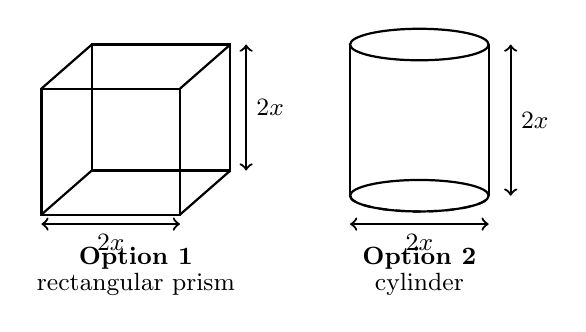
\begin{tikzpicture}[x=0.8cm,y=0.8cm,line width=0.8pt,font=\small]
  \coordinate (A) at (0,0);
  \coordinate (B) at (2.2,0);
  \coordinate (C) at (2.2,2.0);
  \coordinate (D) at (0,2.0);
  \coordinate (E) at (0.8,0.7);
  \coordinate (F) at (3.0,0.7);
  \coordinate (G) at (3.0,2.7);
  \coordinate (H) at (0.8,2.7);
  \draw (A)--(B)--(C)--(D)--cycle;
  \draw (E)--(F)--(G)--(H)--cycle;
  \draw (A)--(E) (B)--(F) (C)--(G) (D)--(H);
  \node at (1.5,-0.7) {\textbf{Option 1}};
  \node at (1.5,-1.1) {rectangular prism};
  \draw[<->] (0,-0.15)--node[below] {\(2x\)}(2.2,-0.15);
  \draw[<->] (3.25,0.7)--node[right] {\(2x\)}(3.25,2.7);

  \draw (6.0,0.3) ellipse (1.1 and 0.25);
  \draw (4.9,0.3)--(4.9,2.7);
  \draw (7.1,0.3)--(7.1,2.7);
  \draw (6.0,2.7) ellipse (1.1 and 0.25);
  \draw[dashed] (4.9,0.3) arc[start angle=180,end angle=360,x radius=1.1,y radius=0.25];
  \node at (6.0,-0.7) {\textbf{Option 2}};
  \node at (6.0,-1.1) {cylinder};
  \draw[<->] (7.45,0.3)--node[right] {\(2x\)}(7.45,2.7);
  \draw[<->] (4.9,-0.15)--node[below] {\(2x\)}(7.1,-0.15);
\end{tikzpicture}
\end{center}

Option 1: A rectangular prism with a square base

Option 2: A cylinder with the same height as the prism, and diameter equal to the side length of the prism's base

\textbf{Option 1:}

Surface Area: \(2(2x)^2+4(2x)^2\)

Volume: \((2x)^3\)

\textbf{Option 2:}

Surface Area: \(2\pi x^2+2\pi x(2x)\)

Volume: \(\pi x^2(2x)\)

The efficiency ratio is \((SA)/(V)\), where SA represents surface area and V represents volume.

\textbf{Option 1:}
\[
\frac{SA}{V}
=
\frac{2(4x^2)+4(4x^2)}{8x^3}
=
\frac{24x^2}{8x^3}
=
\frac{3}{x}
\]

\textbf{Option 2:}
\[
\frac{SA}{V}
=
\frac{2\pi x^2+4\pi x^2}{2\pi x^3}
=
\frac{6\pi x^2}{2\pi x^3}
=
\frac{3}{x}
\]

The company can now compare the efficiency ratio of the package designs.

Prism: \(\dfrac{3}{x}\)

Cylinder: \(\dfrac{3}{x}\)

In this example, the efficiency ratio of the cylinder is equal to that of the prism. So the company should choose their package design based on other criteria.
}{}

\teacheranswerbox{\IconCheck\ ANSWER KEY}{%
\textbf{Answer key (from source):} The efficiency ratio of the cylinder is equal to that of the prism.

\textbf{Image placeholder (from source):} Two package options: Option 1 is a rectangular prism with a square base; Option 2 is a cylinder with the same height as the prism and diameter equal to the side length of the prism's base.
}

\begin{callout}{\IconMic\ TEACHER SCRIPT}{calloutblue}
1. ``Yesterday we simplified with one factoring move. Today we do multi-step AND interpret in context.''\\
2. Ex 2: ``Factor top: difference of squares \(\rightarrow\) \((2-x)(2+x)\). Factor bottom: \((x-2)(x+5)\). Now --- watch: \((2-x) = -(x-2)\). Cancel. Domain: \(x \ne 2\), \(x \ne -5\). The 2 came from the canceled factor --- it STILL blocks.''\\
3. ``Ex 6: what IS efficiency? It's SA divided by Volume. Build each one, simplify, both land on \(3/x\). Interpretation: as \(x\) grows, the ratio \(3/x\) shrinks --- bigger packages are more efficient.''\\
4. ``Same procedure, new meaning. The math doesn't change --- just what we say about the answer.''\\
5. Release.
\end{callout}

\sectionbanner{EXPLORE --- Think-Pair-Share (35 min)}
\textit{Work with a partner. Practice \#19 is assessment-critical (domain restrictions) --- plan \(\sim\)8 min for it.}

\phasetag{TPS \textperiodcentered{} pure DOK-2 mastery \textperiodcentered{} assessment rehearsal}
\frameworkphaseheader{Explore}{2}{35}{%
\phaseitems{
  \item 6 laps across 35 min.
  \item Laps 1-3: Try-It 6 + \#14 + \#22. Abstract simplification with domain. (5-6 min each.)
  \item Laps 4-5: \#34 + \#37 --- modeling items. Build ratio \(\rightarrow\) simplify \(\rightarrow\) interpret.
  \item Lap 6: \#19 --- the assessment rehearsal. Press on domain restriction from cubic denominator.
  \item Do not give answers. Use sentence frame to press interpretation.
}%
}{%
\phaseitems{
  \item 6 items in order. Abstract forms first (Try-It 6, \#14, \#22), then modeling (\#34, \#37), then assessment rehearsal (\#19).
  \item For \#19: BEFORE simplifying, state all denominator zeros. Then simplify. Then write restriction.
  \item Justify with sentence frame.
}%
}{%
\phaseitems{
  \item What are ALL the denominators across every step? (Not just the final one.)
  \item For modeling items: what does the numerator represent? The denominator?
  \item For \#14: did you catch both restrictions? (Factor completely first.)
  \item For \#19: what's special about a cubic denominator? (May have up to 3 zeros.)
  \item For \#37: interpret your answer --- what does \(x \ne \_\_\_\) mean in context?
}%
}{Solo teacher: 6 laps. Press domain restriction reasoning on every item. \#19 IS the assessment rehearsal.}

\textbf{Bank-item labels (in order):}
\begin{enumerate}[leftmargin=1.6em,itemsep=2pt,topsep=2pt]
  \item Try It 6
  \item Practice \#14
  \item Practice \#22
  \item Practice \#34
  \item Practice \#37
  \item Practice \#19 \IconStar\ ASSESSMENT-CRITICAL
\end{enumerate}

\bankitem{Try It 6 (4-3-tryit-6)}{%
The company compares the ratios of surface area to volume for two more containers. One is a rectangular prism with a square base. The other is a rectangular prism with a rectangular base. One side of the base is equal to the side length of the first container, and the other side is twice as long. The surface area of this second container is \(4x^2+6xh\). The heights of the two containers are equal. Which has the smaller surface area-to-volume ratio?
}{}

\teacheranswerbox{\IconCheck\ ANSWER / ANTICIPATED TALK}{%
\textbf{Answer key (from source):} The efficiency ratio for the prism with the rectangular base is less than that for the prism with the square base.
}

\bankitem{Practice \#14 (4-3-savvas-q14)}{%
Use Appropriate Tools Explain why domain restrictions are necessary to show that the rational expressions \(\dfrac{-6x^2+21x}{3x}\) and \(-2x+7\) are equivalent. What is true about the graphs at \(x=0\) and why?
}{}

\teacheranswerbox{\IconCheck\ ANSWER / ANTICIPATED TALK}{%
\textbf{Answer key (from source):} Sample answer: Domain restrictions are needed because you may not be able to tell just from graphs when two expressions are not equivalent. The graphs of \(y=\dfrac{-6x^2+21x}{3x}\) and \(y=-2x+7\) may look identical, but using the trace feature or a table values, \(y=\dfrac{-6x^2+21x}{3x}\) is undefined at \(x=0\), while \(y=-2x+7\) is equal to 7 at \(x=0\).
}

\bankitem{Practice \#22 (4-3-savvas-q22)}{%
What is the simplified form of the rational expression? What is the domain?

\[
\frac{y^2-5y-24}{y^2+3y}
\]
}{}

\teacheranswerbox{\IconCheck\ ANSWER / ANTICIPATED TALK}{%
\textbf{Answer key (from source):} \(\dfrac{y-8}{y}\) for all \(y\) except 0 and \(-3\).
}

\bankitem{Practice \#34 (4-3-savvas-q34)}{%
Find and simplify the ratio of the volume of Figure A to the volume of Figure B.

\begin{center}
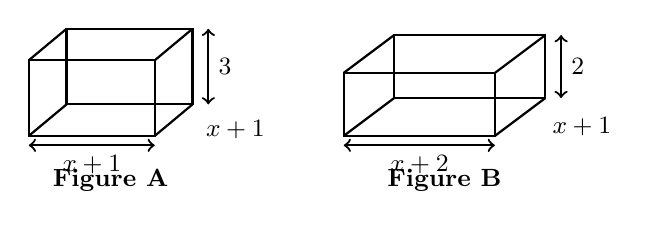
\begin{tikzpicture}[x=0.8cm,y=0.8cm,line width=0.8pt,font=\small]
  \coordinate (A1) at (0,0);
  \coordinate (B1) at (2.0,0);
  \coordinate (C1) at (2.0,1.2);
  \coordinate (D1) at (0,1.2);
  \coordinate (E1) at (0.6,0.5);
  \coordinate (F1) at (2.6,0.5);
  \coordinate (G1) at (2.6,1.7);
  \coordinate (H1) at (0.6,1.7);
  \draw (A1)--(B1)--(C1)--(D1)--cycle;
  \draw (E1)--(F1)--(G1)--(H1)--cycle;
  \draw (A1)--(E1) (B1)--(F1) (C1)--(G1) (D1)--(H1);
  \node at (1.3,-0.7) {\textbf{Figure A}};
  \draw[<->] (0,-0.15)--node[below] {\(x+1\)}(2.0,-0.15);
  \draw[<->] (2.85,0.5)--node[right] {3}(2.85,1.7);
  \node[anchor=west] at (2.65,0.1) {\(x+1\)};

  \coordinate (A2) at (5.0,0);
  \coordinate (B2) at (7.4,0);
  \coordinate (C2) at (7.4,1.0);
  \coordinate (D2) at (5.0,1.0);
  \coordinate (E2) at (5.8,0.6);
  \coordinate (F2) at (8.2,0.6);
  \coordinate (G2) at (8.2,1.6);
  \coordinate (H2) at (5.8,1.6);
  \draw (A2)--(B2)--(C2)--(D2)--cycle;
  \draw (E2)--(F2)--(G2)--(H2)--cycle;
  \draw (A2)--(E2) (B2)--(F2) (C2)--(G2) (D2)--(H2);
  \node at (6.6,-0.7) {\textbf{Figure B}};
  \draw[<->] (5.0,-0.15)--node[below] {\(x+2\)}(7.4,-0.15);
  \draw[<->] (8.45,0.6)--node[right] {2}(8.45,1.6);
  \node[anchor=west] at (8.15,0.15) {\(x+1\)};
\end{tikzpicture}
\end{center}
}{}

\teacheranswerbox{\IconCheck\ ANSWER / ANTICIPATED TALK}{%
\textbf{Answer key (from source):} \(\dfrac{3(x+1)}{2(x+2)}\) for all \(x>0\).
}

\bankitem{Practice \#37 (4-3-savvas-q37)}{%
Look for Relationships A parallelogram with an area of \(\dfrac{3x+12}{10x+25}\) square units has a height shown. Find the length of the base of the parallelogram.

\begin{center}
\begin{tikzpicture}[x=1cm,y=1cm,line width=0.8pt,font=\small]
  \coordinate (P1) at (0,0);
  \coordinate (P2) at (4.0,0);
  \coordinate (P3) at (5.2,2.1);
  \coordinate (P4) at (1.2,2.1);
  \draw (P1)--(P2)--(P3)--(P4)--cycle;
  \draw[dashed] (2.0,0)--(2.0,2.1);
  \draw (1.85,0)--(1.85,0.15)--(2.0,0.15);
  \node[anchor=east] at (1.8,1.05) {\(\dfrac{x+4}{2x+5}\)};
  \node at (3.1,-0.45) {base = ?};
\end{tikzpicture}
\end{center}
}{}

\teacheranswerbox{\IconCheck\ ANSWER / ANTICIPATED TALK}{%
\textbf{Answer key (from source):} The length of the base of the parallelogram is \(\dfrac{3}{5}\) units.
}

\bankitem{Practice \#19 \IconStar\ ASSESSMENT-CRITICAL (4-3-savvas-q19)}{%
Reason If the denominator of a rational expression is \(x^3+3x^2-10x\), what value(s) must be restricted from the domain for \(x\)?
}{}

\teacheranswerbox{\IconCheck\ ANSWER / ANTICIPATED TALK}{%
\textbf{Answer key (from source):} \(-5\), 0, 2
}

\sectionbanner{SHARE / SUMMARY (5 min)}

\phasetag{Concept Summary + LEHS 8-Q preview}
\frameworkphaseheader{Share / Summary}{2}{5}{%
\phaseitems{
  \item Cold-call 1 pair to present \#19 (domain restrictions from cubic denominator).
  \item Project Concept Summary (from student packet).
  \item ``Topic 4 8-Q assessment: expect Q\#2 on THIS content --- domain ID from a cubic. You just rehearsed it.''
}%
}{%
\phaseitems{
  \item Presenting pair uses sentence frame for \#19.
  \item Rest of class signals and annotates their Concept Summary.
}%
}{%
\phaseitems{
  \item What are the TWO big ideas from Lesson 4-3?
  \item If you see a cubic denominator on the assessment, what's the FIRST thing you do?
}%
}{Frame today as assessment rehearsal. Students leave confident on domain restrictions.}

\begin{sentenceframebox}
\textbf{Sentence frames}

Pair share (\#19): ``This ratio compares \_\_\_ to \_\_\_. The rational model is \_\_\_ / \_\_\_. After factoring and canceling, it simplifies to \_\_\_ with \(x \ne \_\_\_\), which means in context that \_\_\_.''

Whole class: one pair reads \#19. Class signals thumbs up/sideways.
\end{sentenceframebox}

\begin{callout}{\IconChart\ CONCEPT SUMMARY (your reference for Topic 4 assessment)}{calloutell}
SIMPLIFYING RATIONAL EXPRESSIONS:\\
\hspace*{1em}\textemdash\ FACTOR numerator and denominator completely.\\
\hspace*{1em}\textemdash\ DOMAIN: exclude ALL zeros of any denominator (original AND intermediate steps).\\
\hspace*{1em}\textemdash\ CANCEL common factors (they still exclude their zeros from the domain).\\
\hspace*{1em}\textemdash\ Write simplified form WITH restriction: e.g., \(-\dfrac{x+2}{x+5}\), \(x \ne 2\), \(x \ne -5\).\\[0.35em]
MODELING WITH RATIONAL EXPRESSIONS:\\
\hspace*{1em}\textemdash\ Name the ratio in words first.\\
\hspace*{1em}\textemdash\ Build each quantity as a polynomial, form the fraction, then simplify.\\
\hspace*{1em}\textemdash\ Interpret the simplified ratio: what do the numerator and denominator mean?\\
\hspace*{1em}\textemdash\ State domain restriction in context (e.g., ``\(x > 0\) because length is positive'').
\end{callout}

\sectionbanner{EXIT}

\phasetag{pre-assessment confidence check}
\frameworkphaseheader{Exit Ticket}{1-2}{3}{%
\phaseitems{
  \item Collect at door.
  \item Tonight: scan for students who can't complete the simplified ratio or restriction. Insert a 5-min Do Now recap when the 8-Q lands.
}%
}{%
\phaseitems{
  \item Complete the three fill-in stems.
  \item Write one biggest thing learned.
}%
}{%
\phaseitems{
  \item Did any student leave the restriction blank?
  \item Did any student interpret correctly but miss the domain?
}%
}{Collect. No grade. Use as data for assessment prep.}

\begin{callout}{\IconClipboard\ EXIT TICKET --- Student Form}{calloutyellow}
A rational model needs factoring because \_\_\_.\\
My simplified ratio is \_\_\_, valid when \(x \ne \_\_\_\).\\
In context this means \_\_\_.\\
One biggest thing I learned today: \_\_\_\_\_\_\_\_\_\_\_\_\_\_\_\_\_\_\_\_\_\_\_\_\_\_
\end{callout}

\sectionbanner{OPTIONAL REINFORCEMENT (not collected)}
\textit{Extra stretch for fast finishers. Try without a calculator first.}

\bankitem{Optional \#1  (Savvas SAT/ACT style)}{%
SAT/ACT For what value of \(x\) is \(\dfrac{2x^2+8x}{(x+4)(x^2-9)}\) undefined?

\begin{center}
\(-8 \qquad -3 \qquad 0 \qquad 4 \qquad 9\)
\end{center}
}{}

\teacheranswerbox{\IconCheck\ ANSWER KEY}{%
\textbf{Answer key (from source):} \(-3\)
}

\clearpage

\begin{callout}{\IconClock\ PERIOD A / PERIOD F --- 65-MIN CLASS NOTES}{calloutpink}
Both sections should have 65 min. Use extra 10 min on Explore \#19 (assessment-critical).\\
If finished early: Practice \#39 (SAT/ACT MC) as fast-finisher stretch.\\
Alternative: project Practice \#22 as a second domain-identification prompt --- more restriction practice.
\end{callout}

\begin{callout}{\IconPuzzle\ MODIFICATIONS / SUPPORT FOR IEP STUDENTS}{calloutiep}
\textbullet\ Provide both Rule cards as half-sheet cut-outs on their desks.\\
\textbullet\ For \#19, provide a pre-factored scaffold showing the denominator already factored so they focus on identifying zeros.\\
\textbullet\ Accept verbal domain restriction identification in lieu of written.
\end{callout}

\begin{callout}{\IconGlobe\ SUPPORTS FOR ELL STUDENTS}{calloutell}
\textbullet\ Sentence frames on student page (don't skip).\\
\textbullet\ Word cards: ``domain'' = allowed \(x\)-values; ``restriction'' = \(x\)-values blocked by division by zero.\\
\textbullet\ ``simplify'' = reduce to lowest terms by canceling common factors.\\
\textbullet\ ``ratio'' = one quantity divided by another (e.g., SA \(\div\) Volume).\\
\textbullet\ Pair ELL students with English-dominant partners for TPS.
\end{callout}

\end{document}
